\chapter{Negative baseline shifts}
\label{cha:np}
During the operation of Siegfried~II inside the GII teststand (see
Chapter~\ref{cha:GII}), a certain class of peculiar events were
observed in significant numbers. The pre-amplifiers and the DAQ system
were configured such, that all channels had positive polarity,
\textit{i.e.}, all signal pulses had to be positive. About 10\% of the
events nevertheless had in at least one segment a negative baseline
shift that could be interpreted as a negative pulse.

\section{Negative pulse events}
\label{sec:np:evt}
Figure~\ref{fig:np:npul} shows a typical ``negative pulse event''. In
this single-segment event all the energy was deposited in
segment~2. The neigboring segments all show mirror pulses as expected
from the weighting potentials. Segment~1, however, also shows a
negative baseline shift. The DAQ should translates this into a
negative energy, but actually sets the value to zero. This causes the
sum of the the energies seen in all segments, $\sum
E_{\text{segment}}$, to be larger than the core energy,
$E_{\text{core}}$. However, would the negative energy be taken into
account, $\sum E_{\text{segment}}$ would be equal to $E_{\text{core}}$
within the resolution.

\begin{sidewaysfigure}[htbp]
\centering
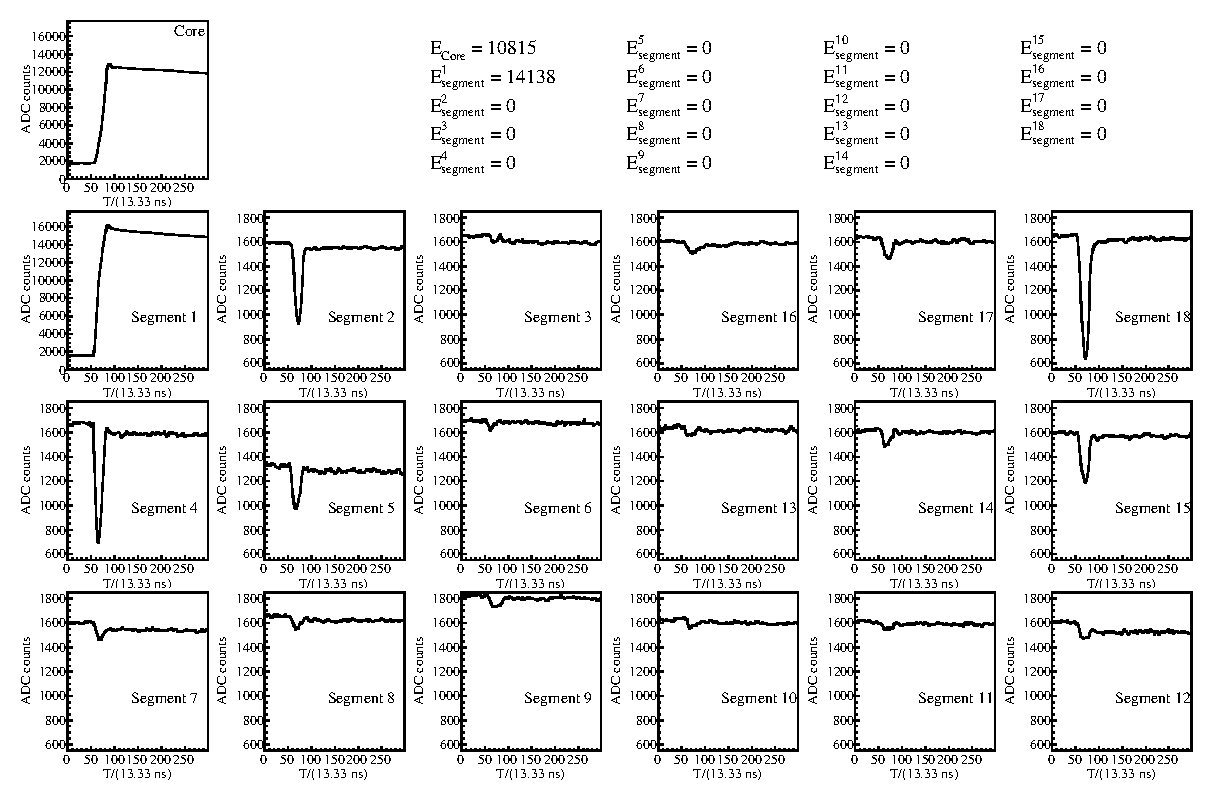
\includegraphics{npul}
\caption{An event showing a negative baseline shift in segment~1. The
energy was deposited in segment~2, mirror pulses are observed in
several segments.}
\label{fig:np:npul}
\end{sidewaysfigure}
The phenomenon cannot easily be interpreted. In the following several
aspects of specially selected events are presented.

\section{Selection of negative pulse events}
\label{sec:np:frac}
Events were selected with $\sum E^{\text{DAQ}}_{\text{segment}} -
E_{\text{core}} > 20\sigma_E$, where $\sum
E^{\text{DAQ}}_{\text{segment}}$ is the sum of the segment energy as
determinde by the DAQ and $\sigma_E$ is the energy resolution.

Figure~\ref{fig:np:sEnegPulse} shows $\sum
E^{\text{DAQ}}_{\text{segment}}$ versus $E_{\text{core}}$ of a data
sample collected with a $^{228}$Th source mounted inside GII on top of
Siegfried II. The two solid lines in the plot indicate the $\pm 20
\sigma$ range around the core energy.

\begin{figure}[tphb]
\centering
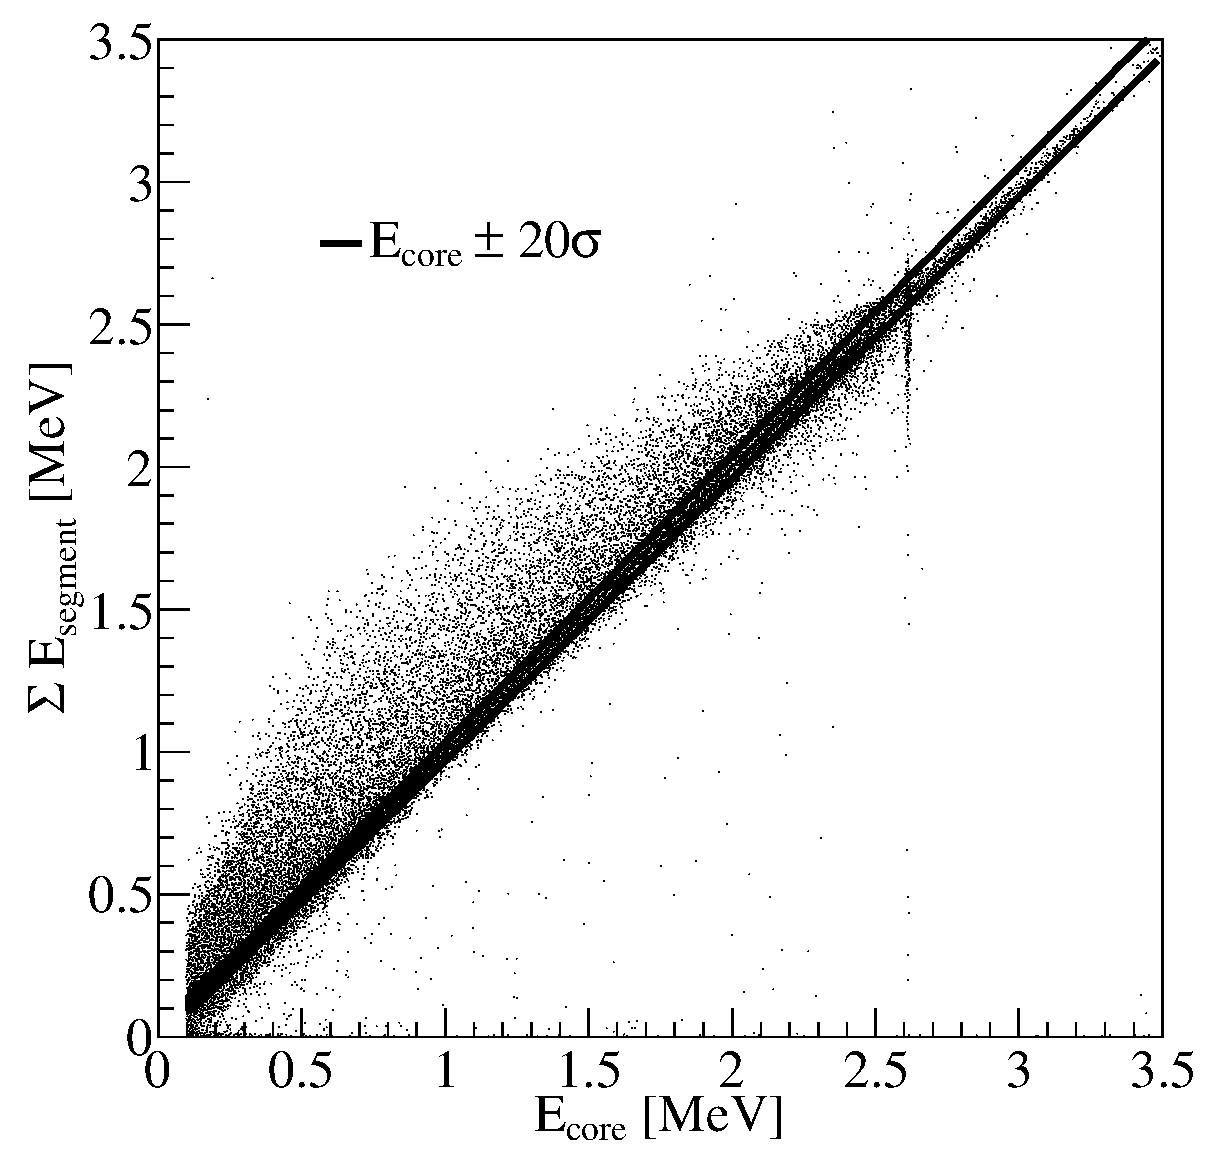
\includegraphics[width=0.5\textwidth]{sEnegPuls}
\caption{Sum of segment energies as determined by the DAQ versus the
core energy. The two solid lines indicate the 20$\sigma$ range around
the core energy.}
\label{fig:np:sEnegPulse}
\end{figure}

Points above the upper solid line correspond to the negative pulse
events. There is also a small fraction of events with$\sum
E^{\text{DAQ}}_{\text{segment}} < E_{\text{core}}$. This is due to
threshold-effects, noise or pile-up, i.e. two pulses are spaced in
time such that the DAQ to cannot provide a correct estimate of the
core and segment energies. As there are quite a number of events with
an energy beyond 2.6~MeV, the pile-up effects are probably
significant.

\section{Location of negative baseline shifts}
\label{sec:np:locneg}

To localize the effect, the individual segment energies were plotted
versus the core energy for the selected
events. Figure~\ref{fig:np:EnegPulse} show that predominantly the top
and bottom segments feature the case $E_{\text{segments}} >
E_{\text{core}}$. Very few negative pulse events were found in the
segments in the middle of the detector.

 
\begin{sidewaysfigure}[tphb]
\centering
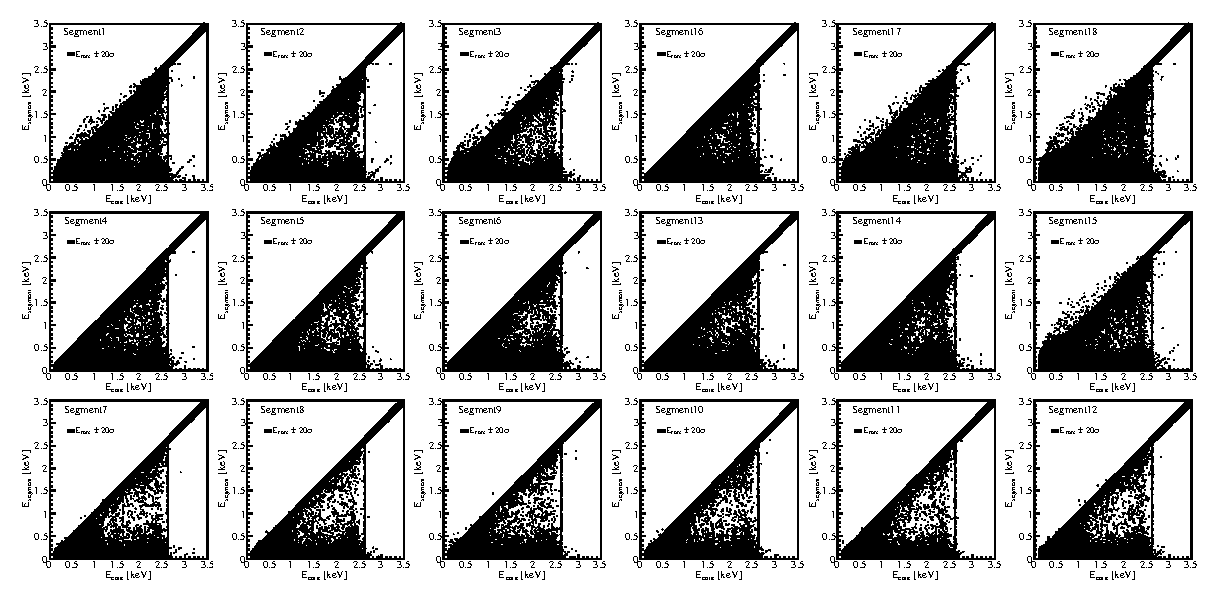
\includegraphics{EnegPuls}
\caption{Energies of individual segments versus the core energy. All
energies were calculated by the DAQ system. The two solid lines in
each plot indicate the $\pm 20 \sigma$ range around the core energy.}
\label{fig:np:EnegPulse}
\end{sidewaysfigure}

\begin{table}[tbhp]
\centering
\caption{Number of negative pulse events in indiviudal segments.
Given are absolute numbers and a ratio to clean single segment
events as determined by the DAQ.} 
\label{tab:np:nenum}
\begin{tabular}{l|rrr|rrr|r} \hline
Top  & 1 & 2 & 3 & 16 & 17 & 18 & total \\\hline
No.($10^{3}$)&$88.5\pm0.3$&$61.2\pm0.2$&$90.7\pm0.3$&$133.6\pm0.4$&$89.0\pm0.3$&$102.7\pm0.3$&$565.7\pm0.8$\\ 
ratio(\%)&$5.34\pm0.02$&$5.28\pm0.02$&$7.31\pm0.03$&$9.24\pm0.03$&$5.47\pm0.02$&$5.73\pm0.02$&$6.34\pm0.01$\\ \hline
Middle& 4 & 5 & 6 & 13 & 14 & 15 & total \\ \hline
No.($10^{3}$)&$1.25\pm0.04$&$1.15\pm0.03$&$0.97\pm0.03$&$1.49\pm0.04$&$2.15\pm0.05$&$1.73\pm0.04$&$8.74\pm0.09$\\ 
ratio(\%)&$0.22\pm0.01$&$0.28\pm0.01$&$0.21\pm0.01$&$0.26\pm0.01$&$0.34\pm0.01$&$0.24\pm0.01$&$0.26\pm0.01$\\ \hline
Bottom& 7 & 8 & 9 & 10 & 11 & 12 & total \\ \hline
No.($10^{3}$)&$18.1\pm0.1$&$11.5\pm0.1$&$15.8\pm0.1$&$14.4\pm0.1$&$13.2\pm0.1$&$17.6\pm0.1$&$90.6\pm0.3$\\ 
ratio(\%)&$3.46\pm0.03$&$3.05\pm0.03$&$3.69\pm0.03$&$2.94\pm0.02$&$2.38\pm0.02$&$2.79\pm0.02$&$3.02\pm0.01$\\ \hline 
\end{tabular}
\end{table}

Table~\ref{tab:np:nenum} lists the numbers for each segment. The
population with negative pulse events is related to the population
with clean single segment events, for which the DAQ found a match
between core and segment energy withing the resolution. The position
of the source is clearly reflected in the differences of numbers of
events between top and bottom and within top and bottom. It was
mounted above the detector and on the side faced by segments 16, 13
and 10.  The ratio to clean single segment events seems constant for
all affected segments.  {\bf or not -- let's see }

The distribution of the risetime of the affected events is shown in
Fig.~\ref{fig:np:nert}. 

\begin{figure}[tphb]
\centering
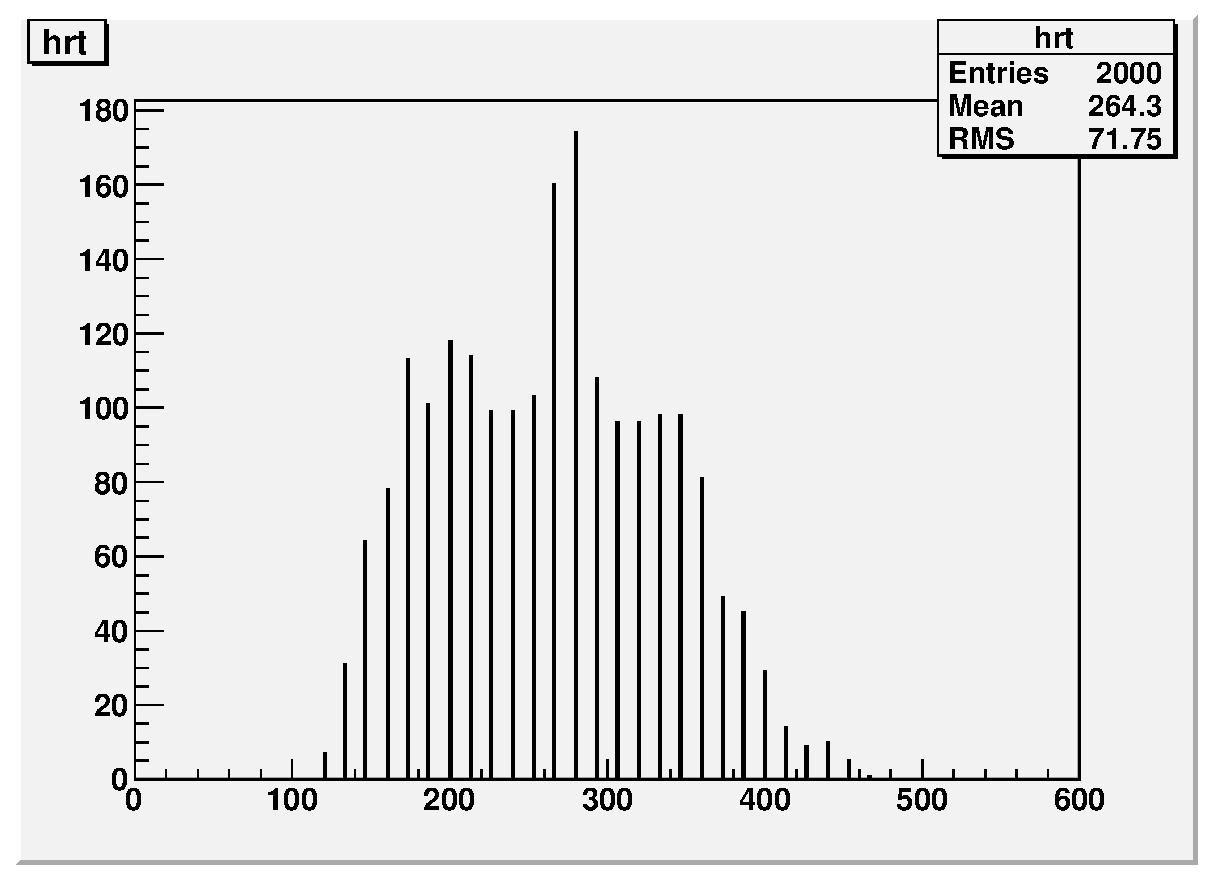
\includegraphics[width=0.45\textwidth]{RTnor}
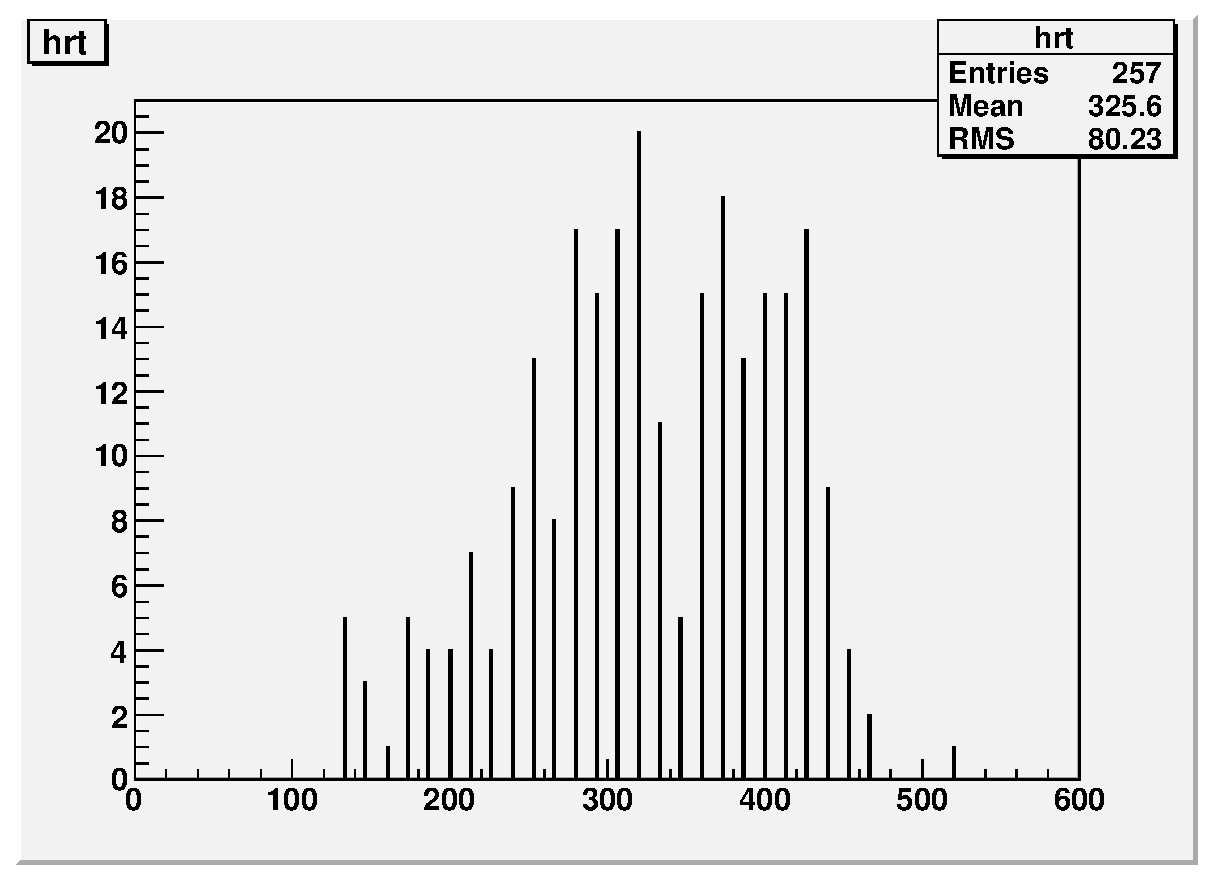
\includegraphics[width=0.45\textwidth]{RTneg}
\caption{Core risetime distribution of events: left, normal events,
right, negative pulse events.}
\label{fig:np:nert}
\end{figure}

\section{Scope}
\label{sec:np:scope}

While the events were observed at a significant rate with
Siegfried~II, some such events also occured in Siegfried~I. There the
rate was, however, well below 1\%. Such events were also observed by
the AGATA detector group [cite -- private communication] again at a
lower rate.

\section{Possible explanations}
\label{sec:np:exp}

\subsection{Grounding}
\label{sec:np:elec}
The grounding scheme for segmented germanium detectors and the
corresponding electronics is delicate. The top and bottom segments
have a different capacitance to the overall gound because the have
adjacent the large detector end surface which does not have a well
defined potential. Siegfried~II did not have its segments fully
metalized, probably enhancing any effect.

Further work on better grounding schemes, especially for the operation
within the GII teststand is under way.


\subsection{Surface channels}
\label{sec:np:surf}

Close to the ends of the detector the formation of surface
channels \cite{Sur05}is expected where the electric field is distorted
and risetimes are expected to increase.

The DAQ energy filter does not handle pulses with extremely long
risetimes correctly and calculates an energy slightly smaller than the
full energy.  This would enhance the event rate on the low energy side
of a full-energy peak at the cost of the peak itself. Such an effect
was seen in Fig.~\ref{fig:ph:mca}: the low energy side of the 1332~keV
peak in data is significantly higher than in the simulation assuming
no field distortion.

However, if the assumption were true, the fraction of negative pulse
events should be larger for low-energy than high-energy photon peaks,
because in average low energy photons deposit their energy closer to
the detector surface.  Events from six photon peaks from the
$^{228}$Th energy spectrum were selected: 239~keV ($^{212}$Pb),
583~keV ($^{208}$Tl), 861~keV ($^{208}$Tl), 2615~keV ($^{208}$Tl) and
its double- and single-escape peaks at 1592~keV and 2103~keV.  For
each of these 6 event samples, the fractions of events with $\sum
E_{\text{segment}} - E_{\text{core}} \gtrsim 20\sigma$ was calculated.
Figure~\ref{fig:np:fracall} shows the result. There is no obvious correlation
between the percentage affected events and photon energy. This does
not support the assumption.

\begin{figure}[tphb]
\centering
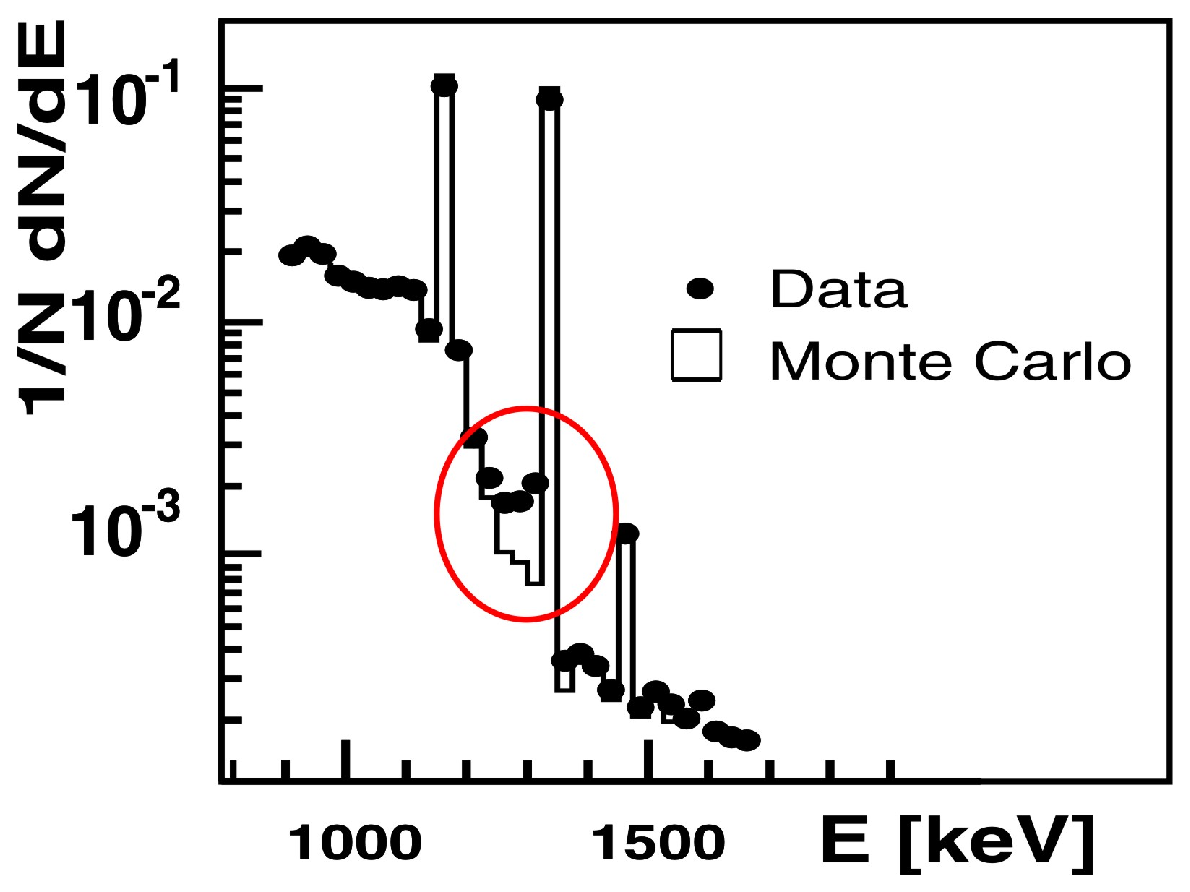
\includegraphics[width=0.4\textwidth]{dmcnew}
\caption{shoulder}
\label{fig:np:shou}
\end{figure}

\begin{sidewaysfigure}[tphb]
\centering
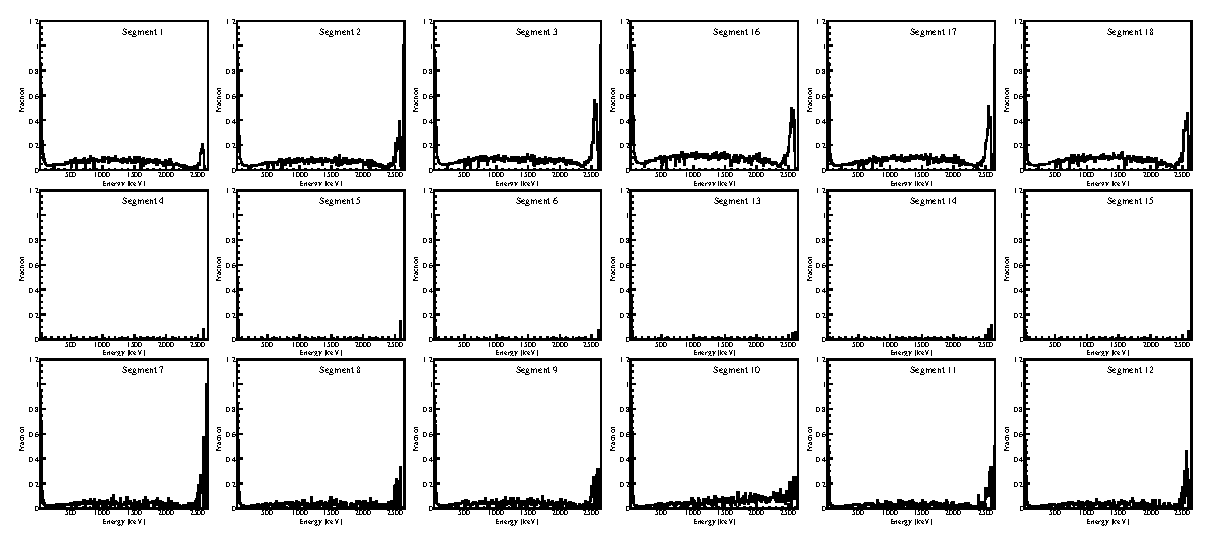
\includegraphics{NegFractionAll}
\caption{Fraction of events with $\sum E_{\text{segment}} -
E_{\text{core}} \gtrsim 10\sigma$ as a function of core energy in all
segments.}
\label{fig:np:fracall}
\end{sidewaysfigure}

\begin{figure}[tphb]
\centering
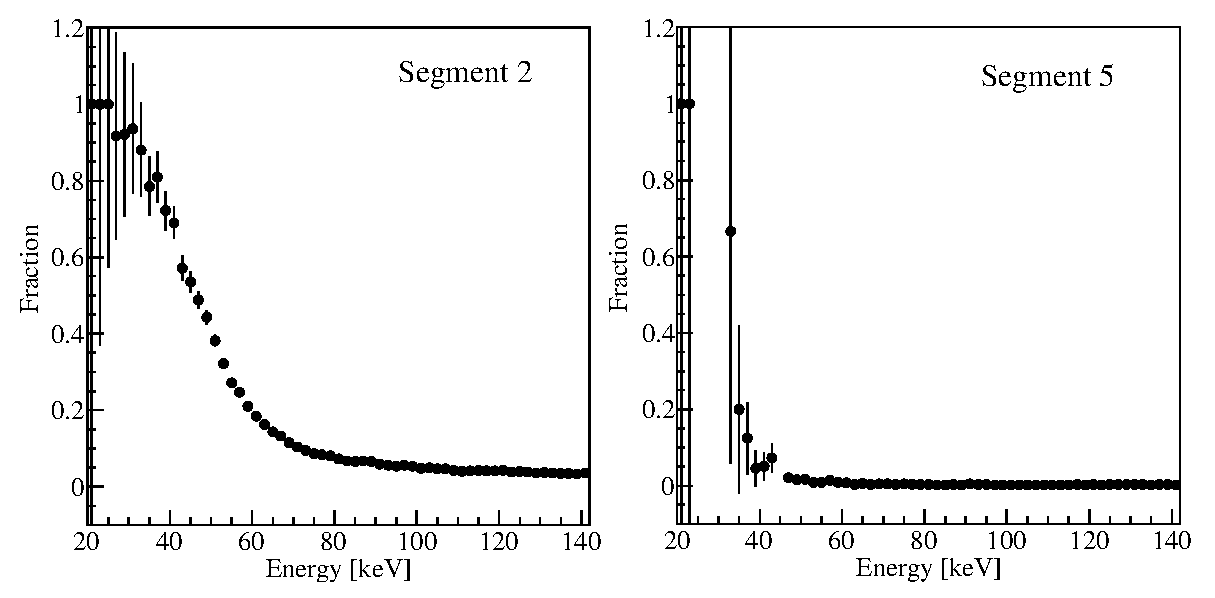
\includegraphics[width=0.6\textwidth]{NegFraction20140}
\caption{Fraction of events with $\sum E_{\text{segment}} -
E_{\text{core}} \gtrsim 10\sigma$ in the low energy region.}
\label{fig:np:fraclow}
\end{figure}

\begin{figure}[tphb]
\centering
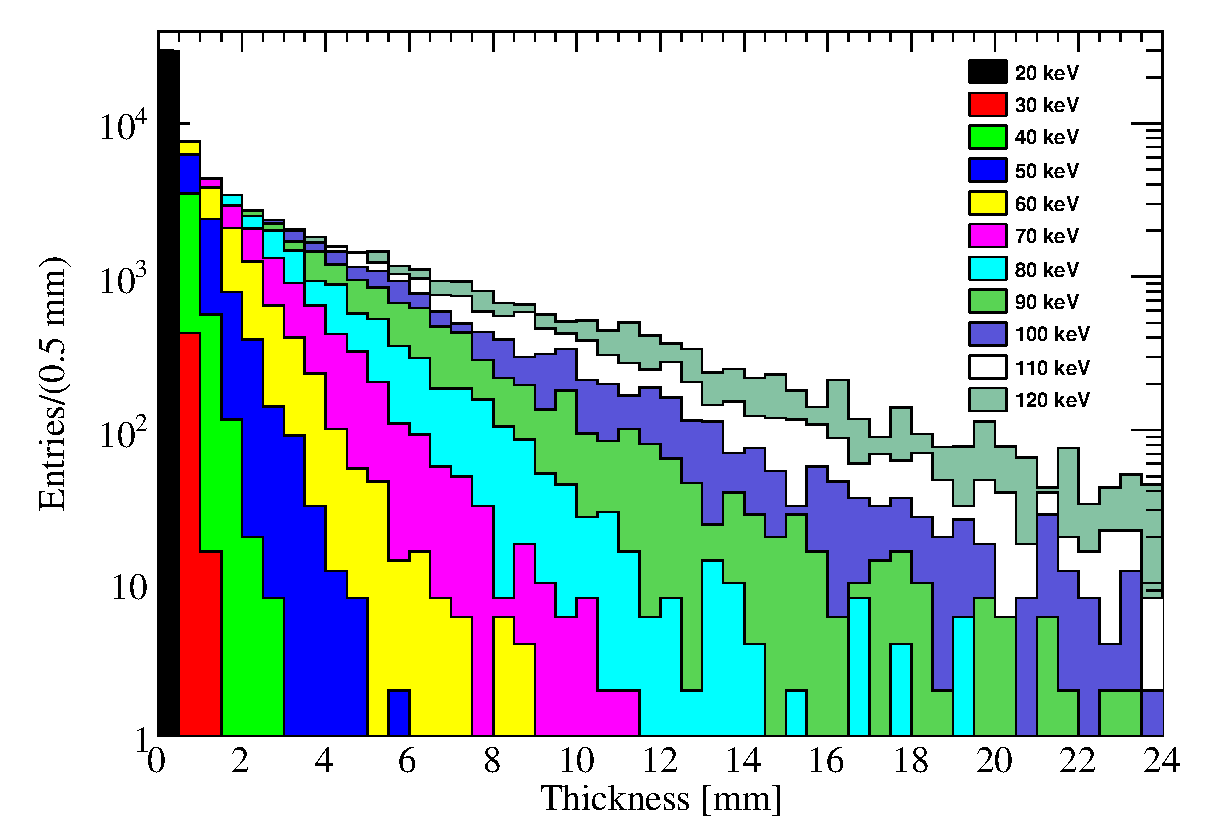
\includegraphics[width=0.6\textwidth]{gDepth}
\caption{Hits distributions created by low energy photons near the
surface of germanium detectors.}
\label{fig:np:gdep}
\end{figure}

\begin{figure}[tphb]
\centering
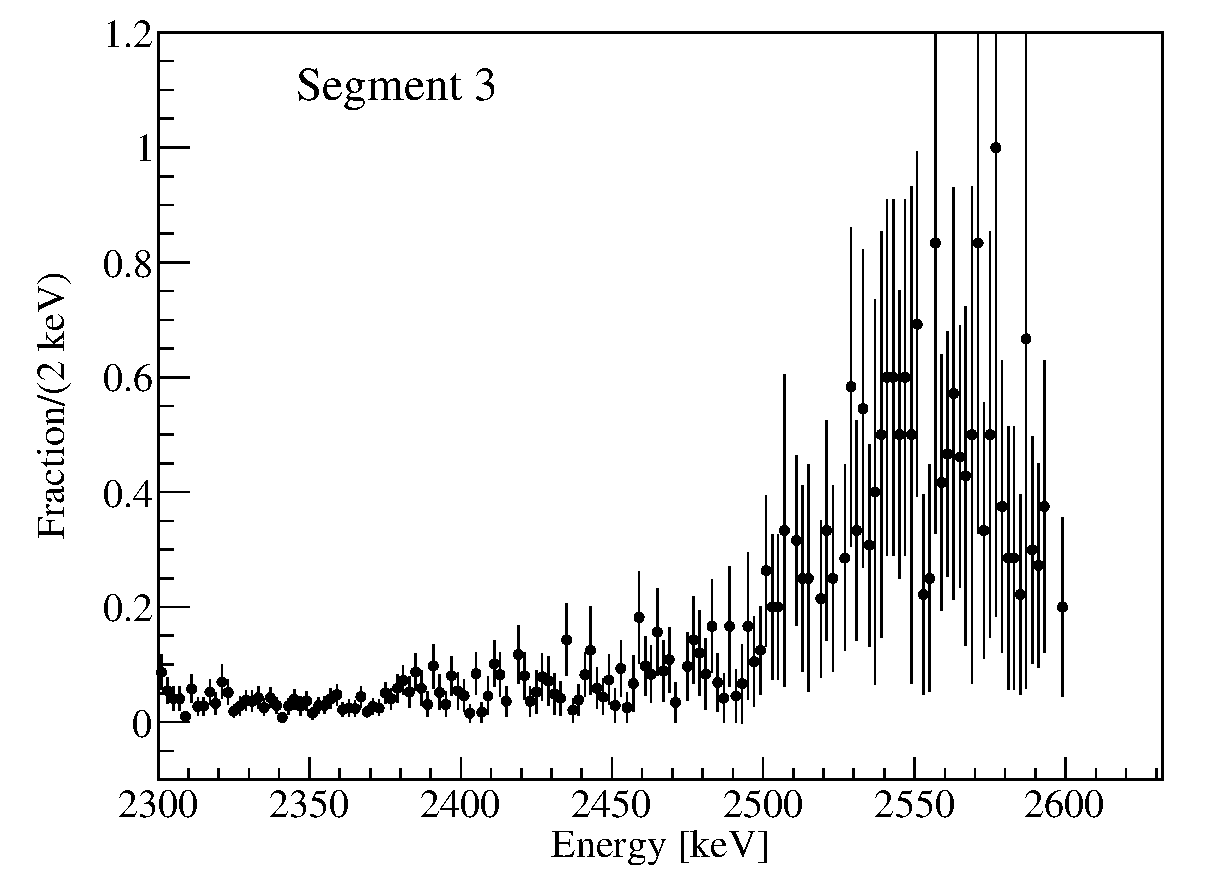
\includegraphics[width=0.6\textwidth]{NegFraction2614}
\caption{Fraction of events with $\sum E_{\text{segment}} -
E_{\text{core}} \gtrsim 10\sigma$ on the low energy side of 2614 keV
peak.}
\label{fig:np:frac2614}
\end{figure}

\section{Summary}
\label{sec:np:sum}
A small fraction of events taken with this setup had segments with
negative baseline shifts which also affected the core energy. The
phenomenon is not yet understood.


%%% Local Variables:
%%% mode:latex
%%% TeX-master: "thesis"
%%% End:
